\documentclass{article}
\usepackage{geometry}
\usepackage[utf8]{inputenc}
\usepackage{graphicx}
\graphicspath{ {images/} }
\geometry{a4paper, left=25mm, right=25mm, top=25mm, bottom=25mm}
\setlength{\parindent}{2em}
\setlength{\parskip}{1em}
\renewcommand{\baselinestretch}{1.3}
\usepackage{fancyhdr}
\pagestyle{fancy}
\fancyhf{}
\rhead{S.Goldie - 42611814}
\lhead{FOAR705 - Learning Journal}
\lfoot{Session 2, 2019 - Macquarie University}
\rfoot{Page \thepage}


% To hyperlink references in contents and other lists
\usepackage[colorlinks=true,linkcolor=blue]{hyperref}
\usepackage{hyperref}
% To create a list of labels
% https://tex.stackexchange.com/a/418302/5482
\usepackage{crossreftools}
% Apply filter to list of labels - so that labels from figures are not affected
\newcommand{\includelabelintoc}{Error:}


\title{FOAR705 - Digital Fundamentals}
\author{Sheriden Goldie}
\date{Session 2, Macquarie University}

\begin{document}

\maketitle

\section*{Data Carpentry Exercises}

% create table of contents based on sections/subsections
\tableofcontents

% Create and index of errors
% so the list has a pretty name
\renewcommand
\listoflabelsname{List of Errors}

\crtlistoflabels
\pagebreak

\section{Spreadsheets for Social Sciences}

It is important for researchers to observe good data practices when working with data to ensure that errors, corruption, and misrepresentation are kept to a minimum. 
Good data practices mean that if mistakes are made - they can be found, noticed, and rectified before any analysis is done. This saves time and frustration from the researchers, and those that hope to use their method or findings. 

\textbf{Initial Questions}
\begin{itemize}
    \item How many people have used spreadsheets in their research?
\end{itemize}

I haven't used spreadsheets for my research - but in my previous 'life' i worked in inventory planning and operations. This lead me to using spreadsheets everyday.

\begin{itemize}
    \item How many people have accidentally done something that made them frustrated or sad?
\end{itemize}

I have had the experience of someone messing up my model data for inventory sheets, that was an time-sink to find the issues and to fix. I have also accidentally applied formulas to the wrong cells, which gave me really weird results. 

\subsection{Formatting data tables in Spreadsheets}

\textbf{Responses to Questions}

\begin{enumerate}
    \item With the person next to you, identify what is wrong with this spreadsheet. Discuss the steps you would need to take to clean up the two tabs, and to put them all together in one spreadsheet.
\end{enumerate} 

There are many things wrong with this spreadsheet:
\begin{itemize}
    \item It is difficult that all the data is split across different tables in each tab - it is hard to tell if the studied locations overlap or not. 
    \item Terms in columns vary - eg. \begin{verbatim} mabati_sloping vs. mabatisloping
    \end{verbatim}
    \item Some data doesn't make sense - eg. -99 in the rooms column - this is not a full integer and is not a valid data point. 
    item\ Data tables are not the same in both tabs. There is a 'Plots' table in Mozambique tab, but not in the Tanzania tab.
    \item the highlighted cell is unclear as to the relevance of the additional barn
    \item the asterisk marked data to include a cowshed is unclear
    \item the asterisked data on cows is misleading as it adds the now dead cow to the count that should just be looking at the collected temporally fixed data
    \item the livestock table in the Mozambique tab is VERY problematic. It combines all data in one cell without defining the individual animal counts
    \item the Mozambique livestock table also includes the 'Look after Cows' column which is not consistent/relevant
    \item the livestock table in the Tanzania tab contains empty fields - is this a zero count, or a missing count?
    \item In the Tanzania tab there seems to be an inconsistency with the 'sunbricks' entry - is this different to burntbricks? - how are these forms being classified and named for the purpose of the study?
    \end{itemize}

\subsubsection{Metadata}
\textbf{A Note on Metadata}

Metadata is data about your data. This is the information that is going to tell you what the answer to a query that is in a column is in reply to. This is imperative as human memory is fallible, and you are likely to forget your intentions unless they are noted and recorded explicitly. 

Digital data is designed to be read by machines, but understanding the meaning of the data can only be done by humans, and this is the valuable part of the process. However your data should be understandable to other humans - for the reasons that they might need to try and replicate your results, or they may wish to replicate the model of your study, or even for their own project starting point - being able to understand the data is made more efficient with metadata. 

Considering metadata during both the collection and analysis phases of research is important, especially if your research is to become part of the scholarly record. 

\noindent \textbf{Questions}
\begin{itemize}
    \item Discuss this data with a partner and make a list of some of the types of metadata that should be recorded about this data set. It may be helpful to start by asking yourself, ``What is not immediately obvious to me about this data? What questions would I need to know the answers to in order to analyze and interpret this data?''
\end{itemize}

Types of metadata that should be recorded
\begin{itemize}
    \item The question or prompt that generated each type of response - eg: for no. of members - the question might be: How many people live in this household? or it might be how many people are in your family? these are distinctly different questions
    \item what the expected range or allowable response is - eg: numerical only, between 1-30, yes/no response only
    \item what the terms used in the data mean - eg: muddaub - means the walls are structured using mud daubed over straw. Or definitions like what a 'plot' or 'room' is being defined as. 
\end{itemize}

\subsection{Formatting Problems}

Other problems to consider is the formatting - using the ``mergecell'' function to make the data look ``pretty''.
As this is ``raw data'' its purpose is to organise the data in a way that is effective and able to be manipulated by the program to create relevant, interpret able outputs. 

\subsection{Dates as Data}
\textbf{Separating dates into components}
to do the exercise these are the processes/actions I took:
\begin{enumerate}
    \item Download file
    \item Open file using Microsoft Excel
    \item Identified table to manipulate
    \item Copied table to new sheet - labelled this sheet 'working tab'
    \item Added three columns between columns A and B using insert columns function. These are labelled 'Day', 'Month', and 'Year' respectively.
    \item Entered the following codes into cells b2: =DAY(A2) c2: =MONTH(A2) d2: =YEAR(A2)
    \item I formatted columns B, C, and D, to a number format without decimal places. 
    \item Adding a new line of data just with the 17/11 information meant the data in the year column automatically populated the current year - 2019. 
\end{enumerate}

\subsection{Quality Assurance}
The processes/actions I took:
\begin{enumerate}
    \item Download file
    \item Open file using Microsoft Excel
    \item Copied table to new sheet - labelled this sheet 'working tab'
    \item Select column D
    \item While column is highlighted go to File - Data - Data Tools - Data Validation
    \item In the section tab of the window use the drop-down menu under Allow to select 'Whole Number'.
    \item Under Data select 'between' and enter 1 as the minimum and 30 as the maximum. 
    \item To test this is working, I tried entering '31' in cell D133. I received an error message as expected. 
    \item Go back to the the Data Validation window. In the Input Error tab, I enter a custom input error name and description.
    \item Go back to the the Data Validation window. In the Error Alert tab select style: Warning and input a custom warning. Title: Invalid Entry. Error Message: Entry must be between 1 and 30.
    \item I created an additional rule set for column E. The age range was set as 0 - 120, it should be a whole number and the warning message was set as: Age should be in whole years and between 0 and 120.
    \item I applied an additional data validation to column F. This was to allow a selection from a list of accepted entries. 
    \item I went to the Data Validation Window while the column was selected. In the Setting's tab I selected the following: ``Allow'' was set to ``List''. with ``ignore blank'' and ``in cell dropdown'' checked. 
    \item Then in the ``Source'' field, I typed the entries, separated by a comma and a space. As so "grass, muddaub, burntbricks, sunbricks, cement"
    \item I entered the Input Error as, title: ``Entry must be as per List'', and Error message: ''The entry must be entered as per the following list: grass, muddaub, burntbricks, sunbricks, cement. Use the dropdown menu to select your entry''
    \item I also tried creating a table as the  ``Source'' data in an additional worksheet. This worked - however care must be taken as this would not be preserved if exporting the data to a .CSV file. 
\end{enumerate}

\subsection{Exporting Data}
Save a file in CSV format.
The steps/actions I took:
\begin{enumerate}
    \item Go to: File - Save As
    \item Select folder directory to save file to
    \item Name file and select .CSV as file format.
    \item Click save
    \item As I had created a new tab for my working data I was only able to save that tab as a CSV. This is good to know for purposes of separating raw data, working data, and for versioning and back up purposes as well. 
\end{enumerate}

\subsection{Reflections}
The Data Carpentry exercises were useful as they reminded me of the 'best practice' ways of dealing with data, and the ideals for how it should be recorded to maximise the potential output. 
In my previous  roles in Inventory Planning and Finance Administration, I have worked with data a lot in various settings and for various purposes - so the mechanics of this task was not new or difficult for me, and so I did not encounter any major issues. 
However the process of documenting my learning process concurrent with the activity of learning was new, and it was useful to think through each step of the process as a single function. 

\section{The Unix Shell}

The aim of this exercise is to gain familiarity with using a Unix Shell. 
I have heard of a Unix Shell before, and have seen one used to manage the data for a commission based sales system. However I have never used it, and am interested to see how it actually works. 

\subsection{Setup}
In the setup we download a zip file, and extract the files within it to the desktop. 
The next step is to open a 'terminal' and type a command. 

I am using windows and do not have a native terminal - so I need to download one. The lesson recommends Git for Windows. 

I go to the following website to download the software:
\begin{verbatim}
    https://gitforwindows.org/
\end{verbatim}

I am able to download, install, and open the software successfully. 

\subsection{Introducing the Shell}

We most commonly interact with computers through a \textbf{GUI}; a \textbf{G}raphic \textbf{U}ser \textbf{I}nterface. We can give instructions to a computer through a GUI by a few mouse clicks. While this model is quite intuitive and easy to learn (it has allowed us to become digitally immersed with little technical training), it doesn't scale well to large scale tasks.  

\textbf{The Shell} is a command line interface, (CLI). This is an interface that is based on "knowledge in the head", but is also able to complete repetitive tasks quickly and efficiently.

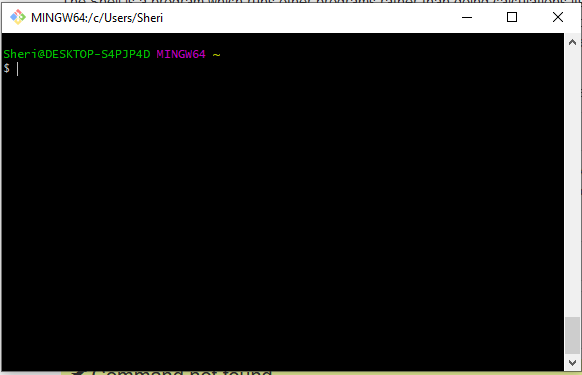
\includegraphics[width=10cm]{Images/GitBash_001.PNG}


The first symbol is \$ - this is a prompt, and means the shell is ready and waiting for you to type a command. 

The first command we try is: ls

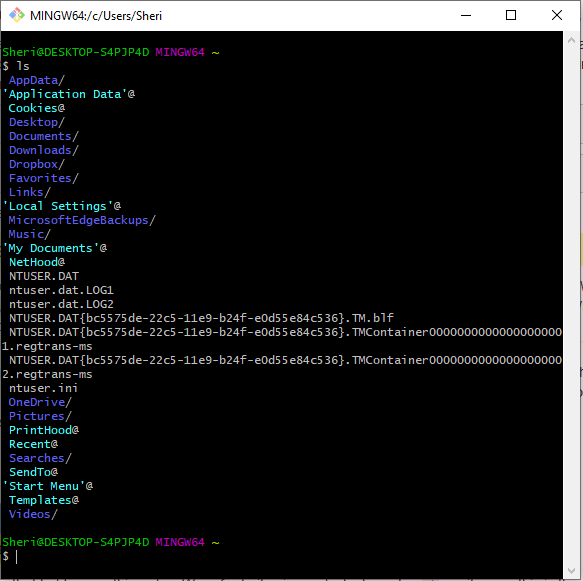
\includegraphics[width=10cm]{Images/GitBash_002.PNG}

This lists the contents of the \textbf{current} directory.
I am able to validate the list generated by the CLI by navigating to the folder using File Explorer in my GUI.
There are some things listed here in light blue that do not appear visibly in my GUI view of the same location.
Later notes indicate that an \@ means a link, an \* means an executable file, and a trailing / means that this is a directory.

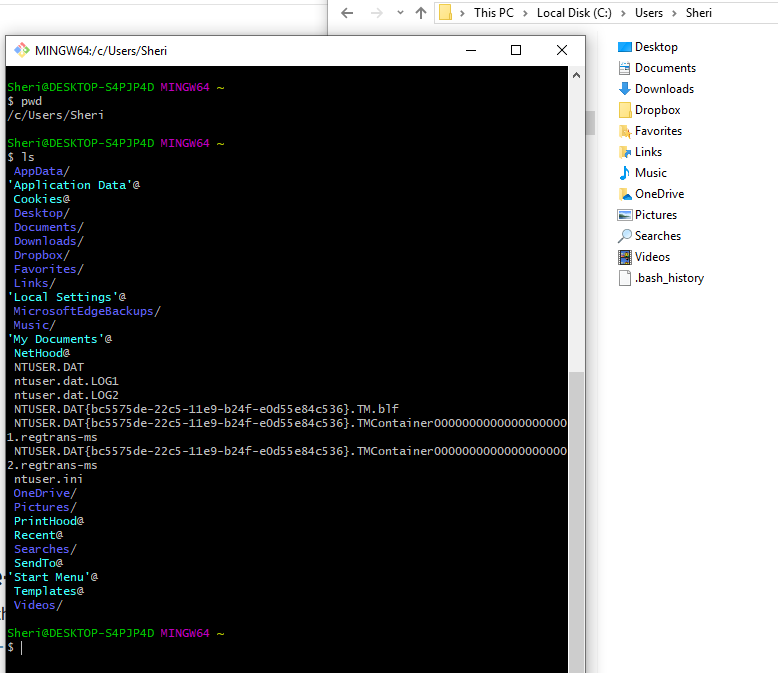
\includegraphics[width=10cm]{Images/GitBash_004.PNG}


\subsection{Navigating Files and Directories}

The first command I use is ``pwd''.
This tells us where we are currently "located in our system according to the CLI. This is important to know, so that we know what locations commands can and will be applied to.

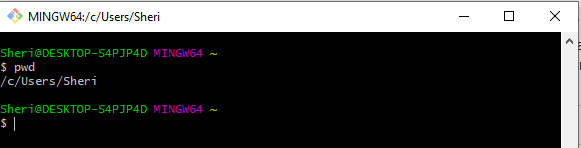
\includegraphics[width=10cm]{Images/GitBash_003.PNG}

\subsubsection{Syntax of a Command Line}
A command line is made up of component parts. For example the following command line: \$ ls -F /

\begin{itemize}
    \item \$ is the prompt beginning all lines in the CLI (At least within GitBash)
    \item ls is a LIST command, and tells the CLI to list everything in a directory
    \item -F is an option (also called a flag or switch) that changes what the command does - in this case it changes the format/colour output.
    \item / is an argument which is telling the command to look to the root directory (not the current directory) to create the list.
\end{itemize}

Options and arguments are also called parameters in some contexts.

Use command ls --help to bring up a list of options for the command. 

Trialling other options:
\begin{itemize}
    \item Command line: ls -l
    \item This creates the list using a ``long'' format. It includes other information about each file/folder.
\end{itemize}

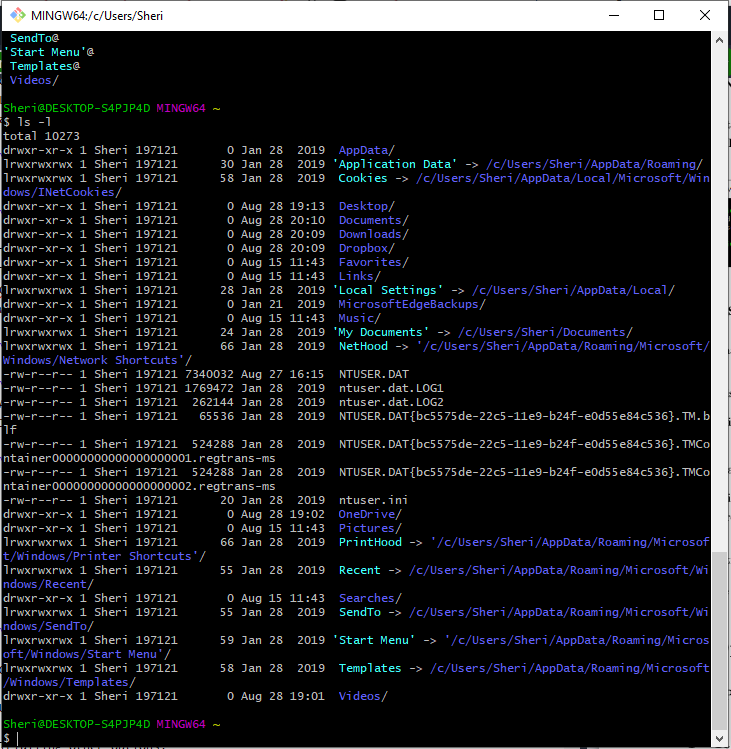
\includegraphics[width=10cm]{Images/GitBash_005.PNG}

\begin{itemize}
    \item Command line: ls -lh
    \item This uses the long list format but simplifies some data points to be more easily readable by a human. 
\end{itemize}

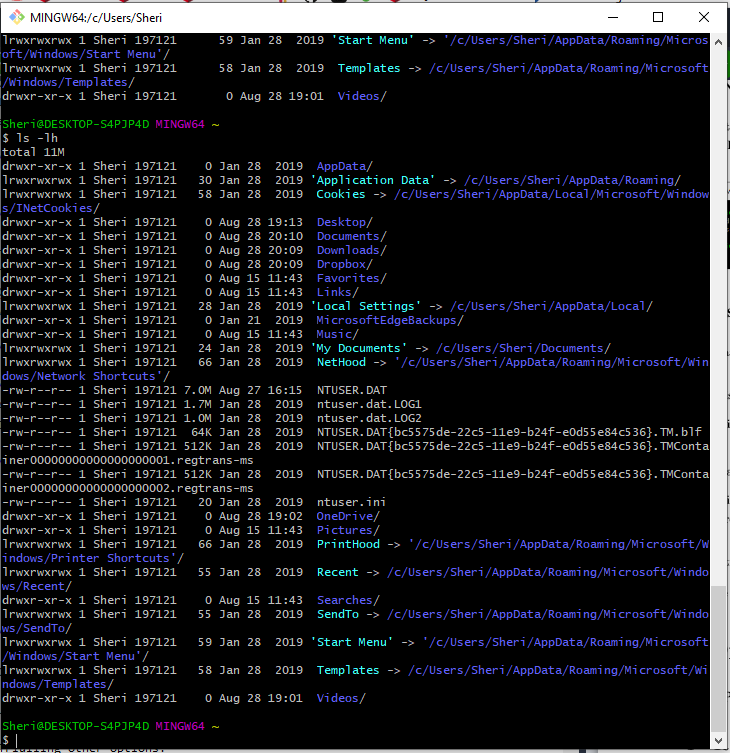
\includegraphics[width=10cm]{Images/GitBash_006.PNG}

The exercise also said to use command line: ls -R which will list the content of the directory recursively. 

When I ran this command - it took a long time to run, as it is listing every directory, and it sub directories and so on at each level. 

Using the option -t shows the list in a different order, based on the last modified folder. 

Next we try moving to different directories using command line: cd [folder location here].

Here cd means change directory - though it really means to change where the shell is considering the current directory to be.

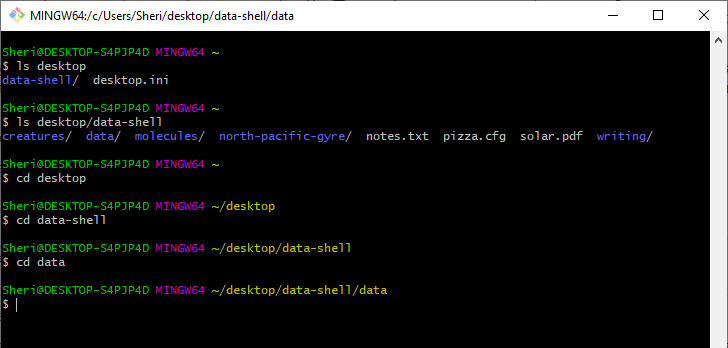
\includegraphics[width=10cm]{Images/GitBash_007.PNG}

Here we can use the pwd command to confirm where we are. Though in GitBash it shows an indication of this in the yellow text.

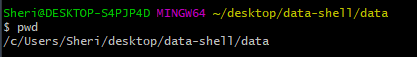
\includegraphics[width=10cm]{Images/GitBash_008.PNG}

If we want to move back through our directories - using cd as we have so far doesn't work, as without any other parameters it is only looking at sub-directories from its current position. 

To move back we use the command cd ..

Here the .. means "directory containing this one".

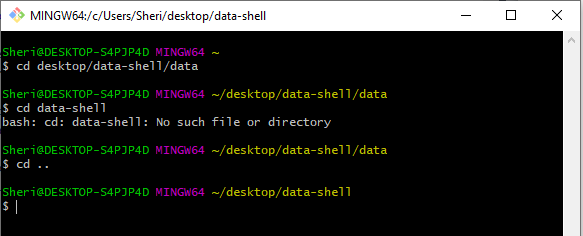
\includegraphics[width=10cm]{Images/GitBash_009.PNG}

We can also add the parameter -a to a ls command to show the indication of these parent directories.

We can also use command cd as a way to return to the root directory. This can then be confirmed by the pwd command.

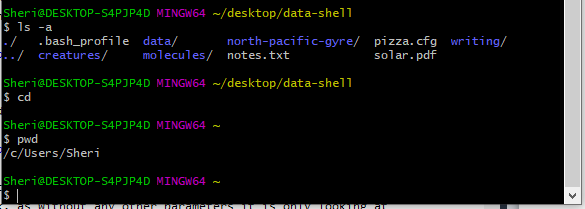
\includegraphics[width=10cm]{Images/GitBash_010.PNG}

Navigate back to the data directory, and validate that you are in the correct place:

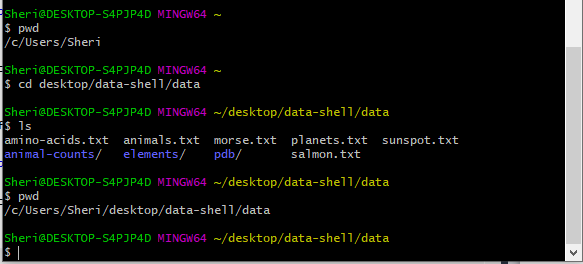
\includegraphics[width=10cm]{Images/GitBash_011.PNG}

\textbf{Other useful shortcuts}

The shell interprets the tilde character (\~{}) at the start of a path to mean ``the current user’s home directory''. For example, if Nelle’s home directory is /Users/nelle, then \~{}/data is equivalent to /Users/nelle/data. This only works if it is the first character in the path: here/there/~/elsewhere is not here/there/Users/nelle/elsewhere.

Another shortcut is the - (dash) character. cd will translate - into the previous directory I was in, which is faster than having to remember, then type, the full path. This is a very efficient way of moving back and forth between directories. The difference between cd .. and cd - is that the former brings you up, while the latter brings you back. You can think of it as the Last Channel button on a TV remote.

\subsubsection{Absolute vs Relative Paths}
So far, when specifying directory names, or even a directory path (as above), we have been using relative paths. When you use a relative path with a command like ls or cd, it tries to find that location from where we are, rather than from the root of the file system.

However, it is possible to specify the absolute path to a directory by including its entire path from the root directory, which is indicated by a leading slash. The leading / tells the computer to follow the path from the root of the file system, so it always refers to exactly one directory, no matter where we are when we run the command.

Source: http://swcarpentry.github.io/shell-novice/02-filedir/index.html

\subsection{Working With Files and Directories}

I first check I am still working in the data-shell directory

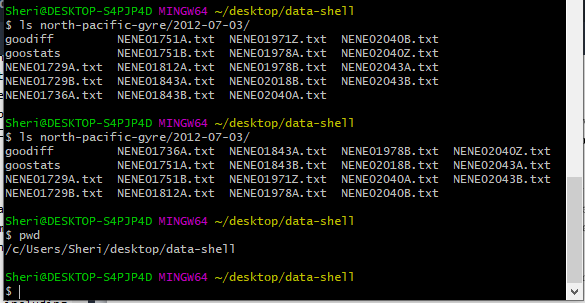
\includegraphics[width=10cm]{Images/GitBash_012.PNG}


\subsubsection{Creating Directories}

To create a new directory within the one we are in, we use the mkdir command:
Validate that the directory has been made using ls command.

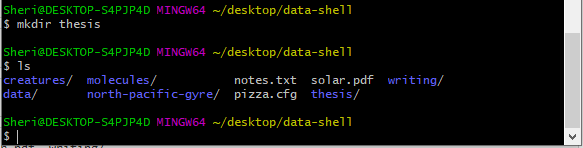
\includegraphics[width=10cm]{Images/GitBash_013.PNG}

\subsubsection{Good Naming Conventions}

For files that you will be using with the CLI - it is important to note that as a ``space'' is what separates commands and parameters, that having spaces in file and directory names is not ideal. Using hyphens, underscores, or using no spaces will make working with files in the CLI much easier.

\subsubsection{Creating a .txt File}

Change the working directory to the newly created ``Thesis'' folder. Create a text file using the command nano.

This will bring up a text editor. Enter some text and use ctrl+o to write the changes to the disc. Use ctrl+x to return to the command line.

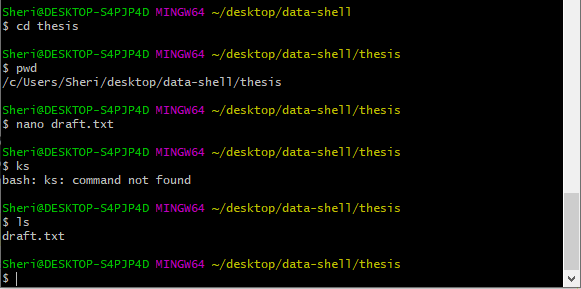
\includegraphics[width=10cm]{Images/GitBash_014.PNG}
\\*
\\*
\textbf{Creating a file a different way}

Try using the touch command to create a .txt file.

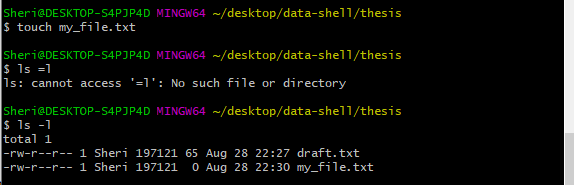
\includegraphics[width=10cm]{Images/GitBash_015.PNG}

This creates the file, but doesn't open the text editor. This creates an empty file. Which is useful for programs that might require a file to be created for it to input data into.

\subsection{Moving Files and Directories}
Return to the data-shell directory.

Change a the file called draft.txt using the mv command.
navigate to the thesis directory and validate that the file has changed names.

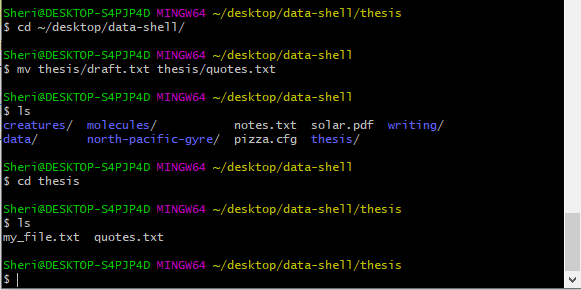
\includegraphics[width=10cm]{Images/GitBash_016.PNG}

Move the quotes.txt file to the current directory using the mv command.
NB: I had to move directories to do this step correctly.

\textbf{Using exact command in CLI error}
\label{ Error: Using exact commands in CLI}

Also including the period . was key for the command to work as this is a shorthand for the current directory.

One has to be careful when specifying the target file name, since mv will silently overwrite any existing file with the same name, which could lead to data loss. An additional option, mv -i (or mv --interactive), can be used to make mv ask you for confirmation before overwriting.

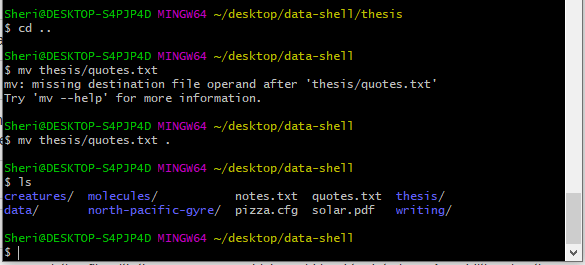
\includegraphics[width=10cm]{Images/GitBash_017.PNG}

\subsection{Copying Files}

Copy the quotes.txt file to the Thesis directory and rename it quotations.txt using the cp command.

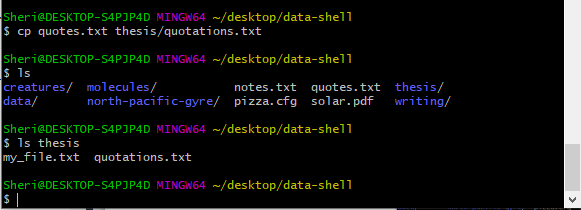
\includegraphics[width=10cm]{Images/GitBash_018.PNG}

You can use the same command on multiple locations in the shell:

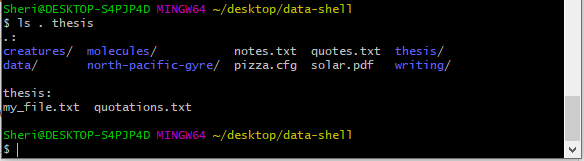
\includegraphics[width=10cm]{Images/GitBash_020.PNG}

Use a recursive option to copy a directory and all it's contents to a different directory.

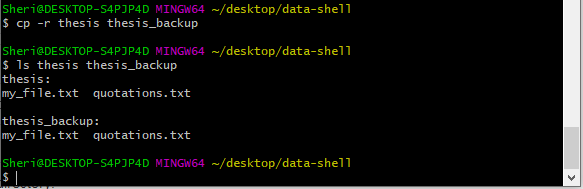
\includegraphics[width=10cm]{Images/GitBash_021.PNG}

\subsubsection{Removing Files and Directories}
Return to the data-shell directory and remove the quotes.txt file using the rm command.

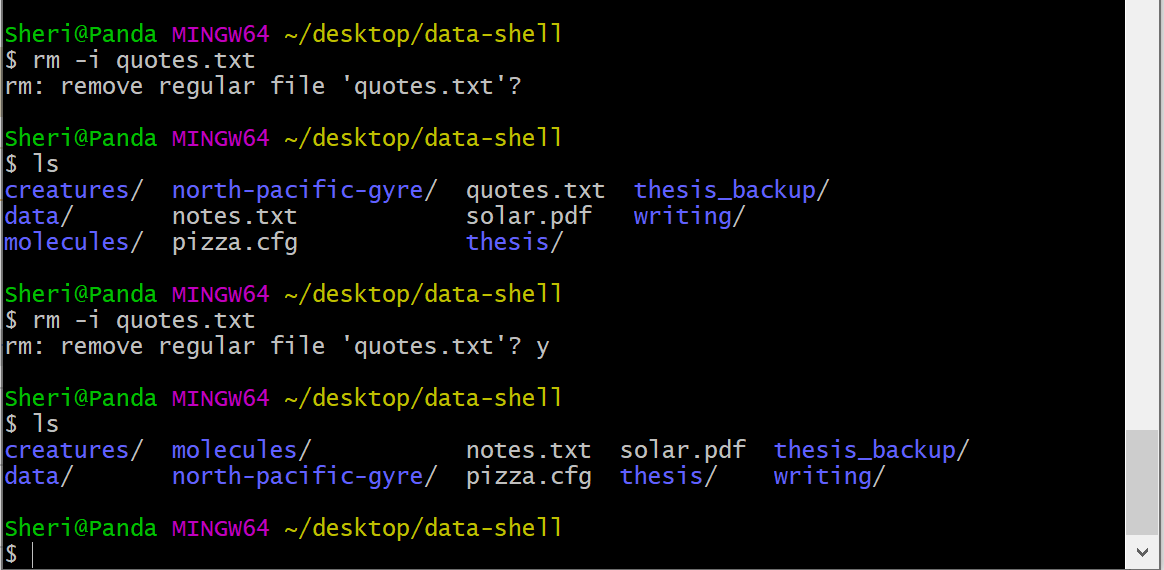
\includegraphics[width=10cm]{Images/GitBash_025.PNG}

\textbf{Shell Command rm -i Confirmation}
\label{ Error: Shell Command rm -i Confrimation}
When using the rm command with the -i parameter, it gives a second prompt to confirm if you want to complete the action. 

This requires a response - as just pressing enter negates the command. I responded by typing y, and this confirmed the command, and removed the file.

When trying to apply this same command to a directory we get an error message.
When using the command rm -ir we are asking to remove the files recursively. So the interface is able to interpret the intention to check/delete the files within the directory. Only when  the directory is empty can it be deleted.

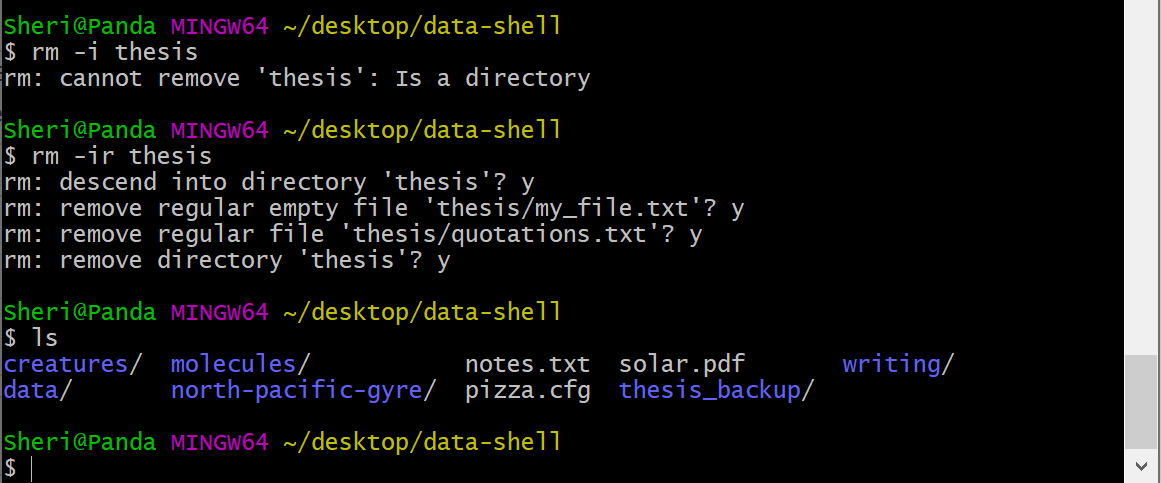
\includegraphics[width=10cm]{Images/GitBash_026.PNG}

\subsubsection{Wildcards}
* is a wildcard function that matches zero or more characters, while ? is a wildcard function that matches exactly one character.

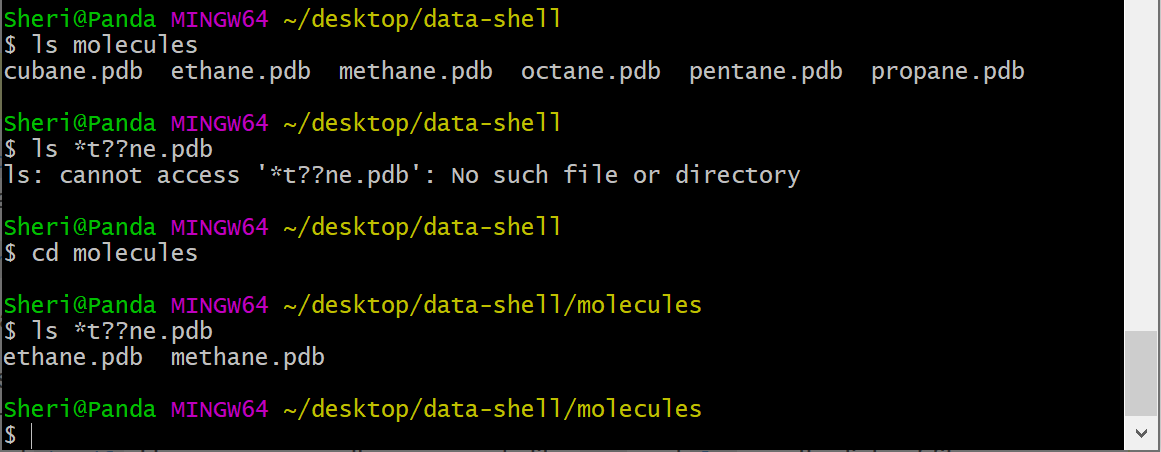
\includegraphics[width=10cm]{Images/GitBash_027.PNG}

\subsection{Pipes and Filters}
We discussed in class that GitBash, or similar Unix shells, are very good at doing individual tasks. The power of it becomes apparent when we are able to combine commands to create an output. This is like putting bits of pipe together, the output of one pipe, one command, can become the input for the next command. 

The first thing in this section is learning the wc command. This is for word count.

The first thing I do is navigate to the necessary location, and verify that I am in the correct place.

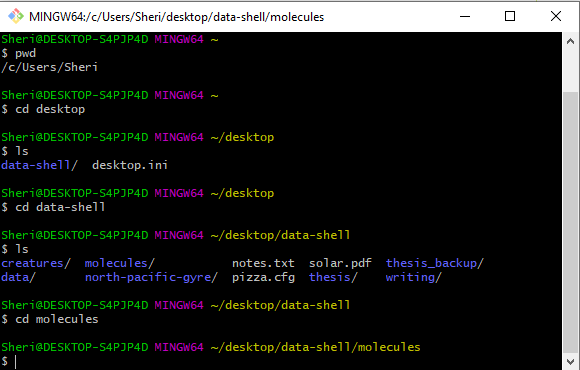
\includegraphics[width=10cm]{Images/GitBash_028.PNG}

The using the wc command, we are able to generate a list. The results from left to right read, line count, word count, character count, filename.

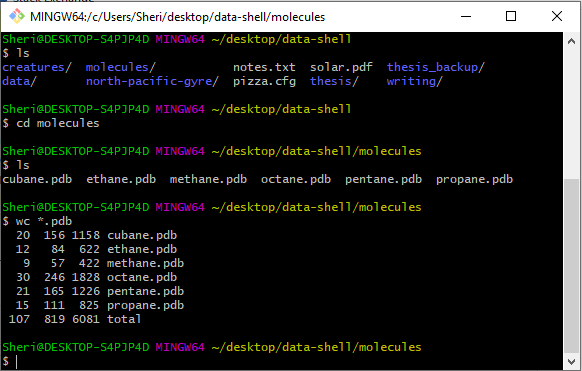
\includegraphics[width=10cm]{Images/GitBash_029.PNG}

Next we apply the filer -l to the command. I am able to do this quickly by using the up arrow to retrieve my previously entered command, and add the -l filter, instead of typing the whole string.

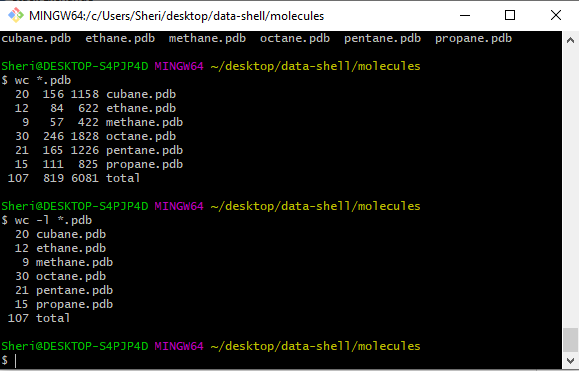
\includegraphics[width=10cm]{Images/GitBash_030.PNG}

We are then able to use the \textgreater{} symbol to redirect the result. Instead of displaying it, it will create a file, which you need to specify the name of.

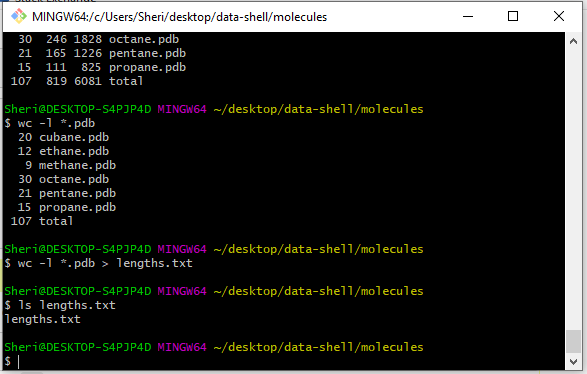
\includegraphics[width=10cm]{Images/GitBash_031.PNG}

Now we can use the sort command on the file we just created. The exercise also asked to use the -n filter to sort the output numerically. However it appears that GitBash automatically sorts numerically in ascending order. 

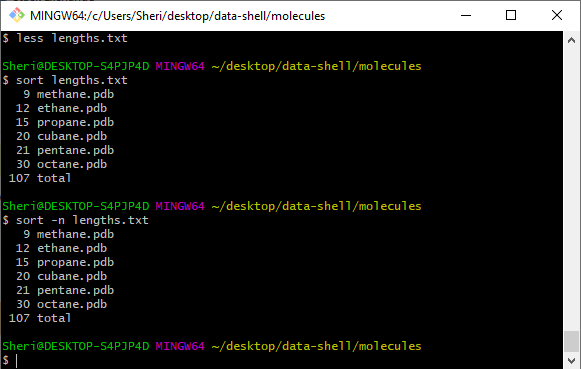
\includegraphics[width=10cm]{Images/GitBash_032.PNG}


Then we can combine this with previous commands to create a new file of the sorted data. We can also use the command, head, to return the heading, or the top rows, according to what we specify.

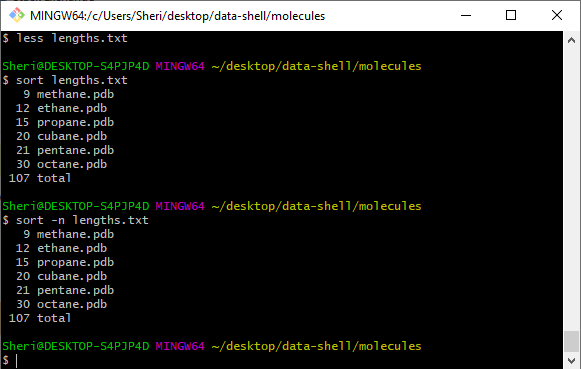
\includegraphics[width=10cm]{Images/GitBash_032.PNG}

There is advice to not try to redirecting the output onto the file that is being worked on. So I tested this. 

This is my lengths.txt file before any changes.

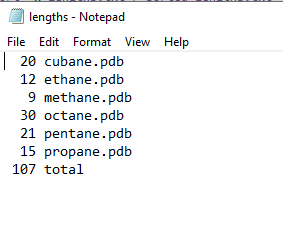
\includegraphics[width=8cm]{Images/GitBash_034a.PNG}

This is the command I ran.

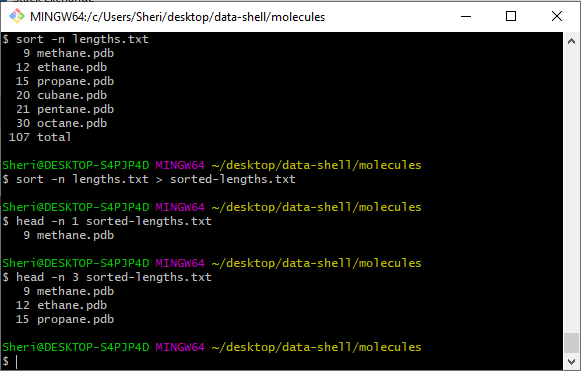
\includegraphics[width=10cm]{Images/GitBash_033.PNG}

This is how the file appeared after this.

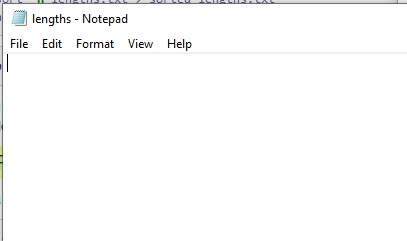
\includegraphics[width=8cm]{Images/GitBash_034.PNG}

The file was empty, the data inside it had been lost. 

\textbf{Using \textgreater{} \textgreater{}}

Using one \textgreater{} sends the output data to a file. \textgreater{}\textgreater{} works slightly differently.

To show this, I followed the exercise and entered the following commands:

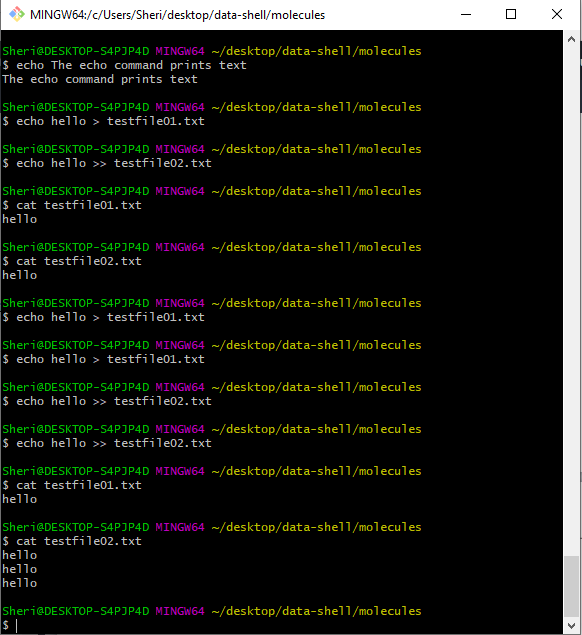
\includegraphics[width=10cm]{Images/GitBash_035.PNG}

This shows that as I entered the commands three times, the use of the \textgreater{} would overwrite the file contents, while the \textgreater{}\textgreater{} would add the new information to the existing file.

Using the | symbol, called pipe, we can combine a number of commands in sequence. 

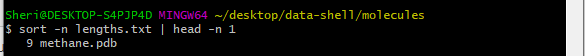
\includegraphics[width=10cm]{Images/GitBash_036.PNG}

We can combine more than two. 

Thinking through the sequence of operations is important. In the last command here, we needed to find the 3 files with the least number of lines in this directory. 

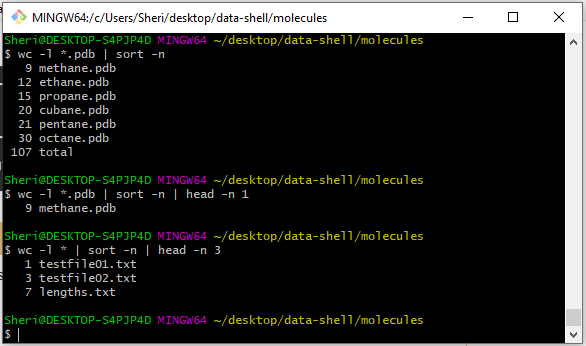
\includegraphics[width=10cm]{Images/GitBash_037.PNG}

We can validate this is correct as there is only a small number of files at this stage using ls - but it is best to be certain of the logic of the string, especially as the data sets get larger.

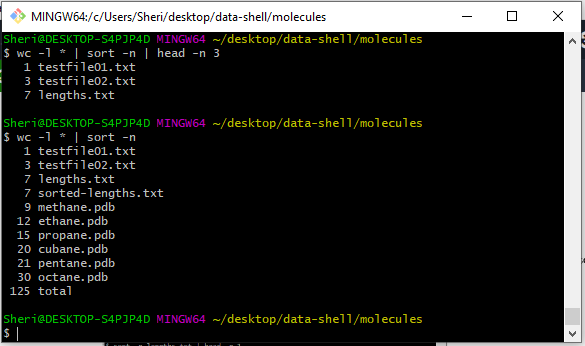
\includegraphics[width=10cm]{Images/GitBash_038.PNG}

\textbf{Pipe Reading}
In the pipe reading exercise - we must read the commands, and figure out what happens, to what data in each step.

I found this easiest when I segmented each step - and focused on the fact that the output of one command became the input for the next. 

I believe I will end up with the rows of data ending, rabbit, deer, raccoon. 

These are the strings I followed to check my thinking and outcome. 

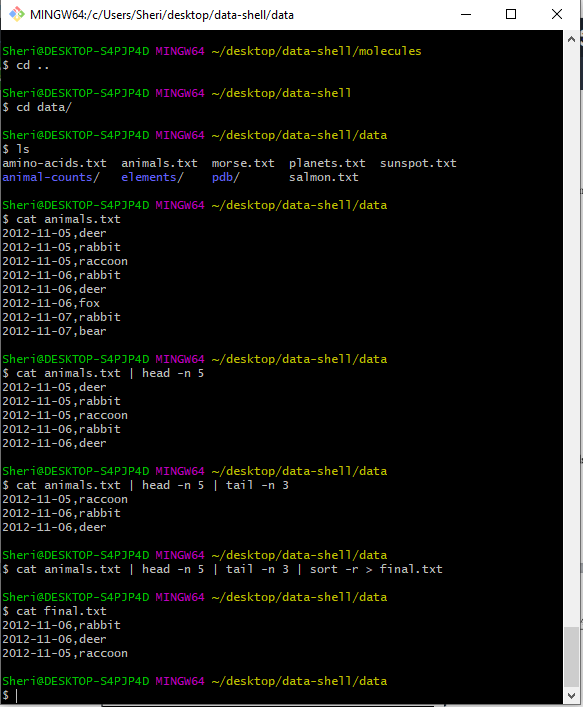
\includegraphics[width=10cm]{Images/GitBash_039.PNG}

\textbf{Pipe Construction}
In the pipe construction, we are shown the commands that will extract/isolate parts of the data we refer to. 
We then are asked to formulate a string to achieve creating a list of the unique animals listed in the file animals.txt

This is my working:

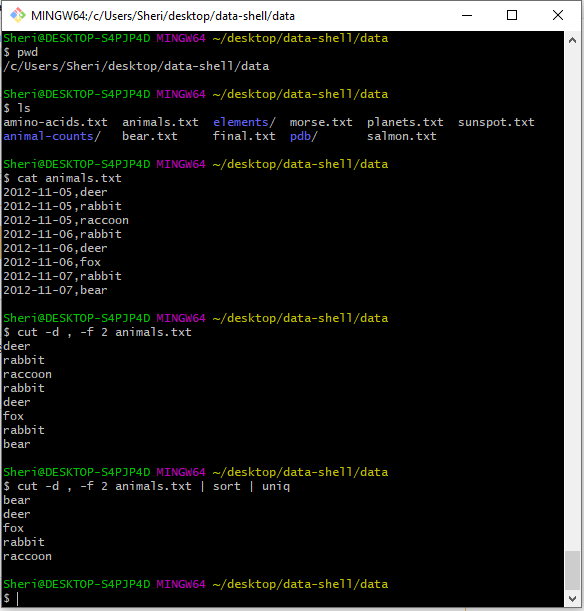
\includegraphics[width=10cm]{Images/GitBash_040.PNG}



\section{OpenRefine for Social Sciences}
\subsection{Part 1}


\section{R for Social Sciences}
\subsection{Part 1}


\end{document}
